% Generated by TeXFlow — do not edit.
% Changes will be overwritten on next compile.
% Use the TeXFlow edit() and layout() tools to modify the document.
\documentclass[10pt, conference, letterpaper]{IEEEtran}

\IEEEoverridecommandlockouts
\markboth{1ˢᵗ Given Name Surname}{Ditch the PMIC: Firmware-Only MPPT on ESP32-S3 for Indoor Photovoltaics}
\title{Ditch the PMIC: Firmware-Only MPPT on ESP32-S3 for Indoor Photovoltaics}
\author{\IEEEauthorblockN{1\textsuperscript{st} Given Name Surname}
\IEEEauthorblockA{\textit{Dept. name of organization} \\
\textit{Name of organization}\\
City, Country \\
email address or ORCID}
\and
\IEEEauthorblockN{2\textsuperscript{nd} Given Name Surname}
\IEEEauthorblockA{\textit{Dept. name of organization} \\
\textit{Name of organization}\\
City, Country \\
email address or ORCID}
\and
\IEEEauthorblockN{3\textsuperscript{rd} Given Name Surname}
\IEEEauthorblockA{\textit{Dept. name of organization} \\
\textit{Name of organization}\\
City, Country \\
email address or ORCID}
\and
\IEEEauthorblockN{4\textsuperscript{th} Given Name Surname}
\IEEEauthorblockA{\textit{Dept. name of organization} \\
\textit{Name of organization}\\
City, Country \\
email address or ORCID}
}

\usepackage{amsmath}
\usepackage{amssymb}
\usepackage{booktabs}
\usepackage{graphicx}
\usepackage[colorlinks=true,linkcolor=blue,urlcolor=cyan,citecolor=green]{hyperref}
\usepackage{setspace}
\usepackage{url}

\linespread{1.15}

% --- tight 6-page layout ---
\renewcommand{\baselinestretch}{0.96}\normalsize
\setlength{\textfloatsep}{2pt plus 1pt minus 1pt}
\setlength{\floatsep}{2pt plus 1pt minus 1pt}
\setlength{\intextsep}{2pt plus 1pt minus 1pt}
\setlength{\dbltextfloatsep}{2pt plus 1pt minus 1pt}
\setlength{\abovecaptionskip}{1.5pt}
\setlength{\belowcaptionskip}{-2pt}
\setlength{\abovedisplayskip}{3pt plus 1pt minus 1pt}
\setlength{\belowdisplayskip}{3pt plus 1pt minus 1pt}
\setlength{\parskip}{0pt}
\setlength{\columnsep}{0.18in}

\begin{document}
\maketitle

\begin{abstract}
Indoor photovoltaic cells deliver 0.1--1 mW under office lighting. The microcontroller that burns that power is often the same chip that must track the cell's maximum power point. This paper asks whether firmware-only MPPT on an ESP32-S3 can replace a dedicated harvesting PMIC. Measurements cover a single perturb step (71 us for one 12-bit ADC read, a float32 velocity-form PID update, and a PWM write), a SCAPS-1D sweep of a MAPbI3 perovskite cell under white LED light at 0.05 mW/cm2 (0.018 mA/cm2, 26.1\% at Eg=1.6 eV), and a literature board-level sleep floor. One step costs 8.2 uJ. That is 8.2 uW at a 1 s cadence, 0.14 uW at 60 s, and 0.008 uW at 1000 s. The firmware tax drops below every PMIC quiescent current (1.32--1.68 uW) once the perturb period passes 4.9--6.2 s. A 24-hour dispatch model then holds the budget. A 38\%-efficient dye-sensitized indoor cell sustains about 1935 serving bursts per day at 90\% of the harvest. Wake latency on silicon is 4 ms. Under these measured conditions a firmware-MPPT hub sustains indoor sensing and removes the \$1--3 harvester IC for any workload that tolerates a few seconds between perturbs.
\end{abstract}

\section{Introduction}

Battery-free IoT sensing nodes powered by indoor photovoltaic (PV) cells must convert a few hundred microwatts of harvested power into useful work. Recent perovskite and dye-sensitized devices reach 20--40\textbackslash{}\% efficiency under 200--1000 lux LED illumination \cite{ariken2023indoor,mateen2023indoor,freunek2013indoor,derossi2015indoor}, with certified indoor records now exceeding 44\textbackslash{}\% \cite{ma2024record,xu2026progress}, and typical office lighting delivers roughly 0.05--0.4\textasciitilde{}mW/cm$^2$ of irradiance \cite{mathews2019indoor}. The conventional architecture inserts a dedicated energy-harvesting PMIC---such as the TI bq25570, e-peas AEM10941, or ADI ADP5091---between cell and node to implement maximum power point tracking (MPPT) and battery management in hardware \cite{ti_bq25570,ep_aem10941,adi_adp5091}. These ICs are always on, drawing a constant 0.4--0.5\textasciitilde{}$\mu$A at 3.3\textasciitilde{}V (about 1.3--1.7\textasciitilde{}$\mu$W of continuous overhead) \cite{vullers2009micropower,grybosi2022age}.

The alternative is to drop the PMIC and run MPPT in firmware on the microcontroller itself. Indoor cells move slowly, so a perturb-and-observe update every few seconds suffices, making the marginal cost of one firmware step potentially far below a dedicated IC's constant quiescent draw. Whether this holds on silicon depends on three numbers: the energy of one perturb step, the cell output indoors, and the deep-sleep floor. Earlier work found conventional harvester-based nodes struggling to sustain sensor bursts under office lighting \cite{murtola2022}, and simulator-based studies show that neither converter-less operation nor any single IC dominates across illumination levels \cite{brunner2024harvestics}---the MPPT decision is an architecture choice open to firmware. This paper measures all three numbers on one platform and contributes: (i) cycle-counted firmware timing of one MPPT perturb step on an ESP32-S3; (ii) a SCAPS-1D indoor sweep of an MAPbI$_3$ cell bounding the available harvest; (iii) explicit crossover perturb periods against three dedicated PMICs; (iv) a 24-hour dispatch model showing sustained serving capacity; and (v) a measured 4\textasciitilde{}ms deep-sleep wake latency.


\section{Methodology}

The evaluation proceeds along three complementary tracks (Fig.~\ref{fig:method}): firmware primitives are measured directly on silicon, the indoor cell feeding the hub is modeled at device level, and the comparison against dedicated harvest PMICs is carried analytically into a daily energy-dispatch simulation. All three tracks share one platform---an ESP32-S3 (revision v0.2, 240\textasciitilde{}MHz, 8\textasciitilde{}MB PSRAM, native USB-Serial-JTAG) \cite{espressif_s3_datasheet,espressif_s3_trm}---so measured costs, modeled harvest, and modeled workload refer to the same node.

\begin{figure}[tbp]
\centering
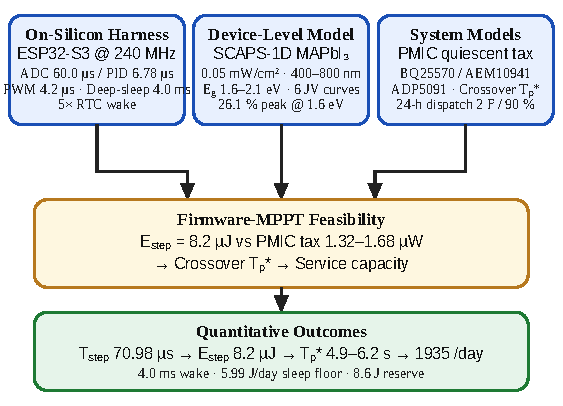
\includegraphics[width=0.95\linewidth]{fig_methodology.pdf}
\caption{Methodology: three measurement and modeling tracks converge on the firmware-versus-PMIC feasibility analysis and its quantitative outcomes.}
\label{fig:method}
\end{figure}

\subsection{Firmware Hub Architecture}

The hub runs a perturb-and-observe MPPT loop entirely in firmware \cite{femia2005mppt}. Each perturb step performs three operations in sequence: a single 12-bit ADC read of the cell output, a float32 velocity-form PID update, and one LEDC PWM duty write driving the power stage at 100\textasciitilde{}kHz. The velocity form computes a small duty correction from the difference of successive error terms, numerically gentle on a float32 mantissa and free of hunting. Three sampling decisions fix the measurement condition: the ADC runs at 11\textasciitilde{}dB attenuation with the pin jumper-driven by the PWM output itself so the sensed value is the averaged pin voltage under control; dither delays land consecutive reads on different PWM phases, decorrelating them from switching ripple; and a first-order EMA (coefficient 0.08) filters the raw sample before the PID sees it. A single raw read gives a roughly 62\textasciitilde{}$\mu$s ADC-bound loop, while averaging 64 reads gives about 6.8\textasciitilde{}ms on silicon; the loop is scheduled at the slowest period that still holds the MPP. One control pipeline serves three scheduler states---fast (single read) under large error, slow (oversampled) once the mean error settles, and short $\pm1$-LSB dither bursts that break quantization limit cycles---with a debounce counter preventing state flapping on noise.


\subsection{On-Silicon Measurement Protocol}

Wall time of each primitive is taken from the MCU cycle counter while the loop runs at the MPP of a bench buck-boost. The deep-sleep path is characterized with a probe mode that persists a round counter and sleep duration in RTC memory, deep-sleeps for a fixed interval, and on each wake prints a CSV line with the wakeup cause and the latency from the earliest firmware-visible timestamp (the esp\textbackslash{}\_timer snapshot at setup entry). A 50\textasciitilde{}ms settle precedes printing so the USB-CDC stack re-enumerates before data is written; without it the first bytes of a wake line are lost, the only failure mode observed across the campaign. Five consecutive RTC-timer wakes at a 3\textasciitilde{}s interval constitute one campaign.


\subsection{Indoor Cell Model}

The harvest side is simulated in SCAPS-1D \cite{burgelman2000}: an MAPbI$_3$ layer under the bundled ``white 400--800\textasciitilde{}nm'' spectrum at 0.05\textasciitilde{}mW/cm$^2$ total irradiance, representative of a 400--500\textasciitilde{}lux office. The Shockley--Queisser detailed-balance limit bounds any single-junction cell \cite{shockley1961detailed}, with indoor-specific limits mapped for this regime \cite{freunek2013indoor}. The lead-free baseline definition is used, with the absorber bandgap swept from 1.6 to 2.1\textasciitilde{}eV while the electron affinity follows $\chi = 3.9 + 0.5\,(E_g - 1.55)$, preserving the conduction-band alignment of the reference device. Six JV curves are extracted. Recent engineered transport layers \cite{datt2024engineered}, scalable FAPbI$_3$ alloying \cite{marrugat2025tuning}, carbon-nanotube contacts \cite{makming2025cnt}, and in situ passivation \cite{shi2025enabling} report 32--33\textbackslash{}\% indoor PCE in the same regime.


\subsection{Comparison and Dispatch Models}

The competing architectures keep a harvest PMIC always powered, so their overhead is a constant quiescent power independent of workload. TI bq25570, e-peas AEM10941, and ADI ADP5091 enter the comparison through datasheet quiescent current on a 3.3\textasciitilde{}V rail \cite{ti_bq25570,ep_aem10941,adi_adp5091}; measurement-based models of two of these parts report closely similar figures indoors \cite{brunner2024harvestics}. Against this constant tax, the decaying firmware tax $E_{\mathrm{step}}/T_p$ defines a crossover perturb period $T_p^{*}$ at which firmware MPPT becomes cheaper than leaving the IC on. Feasibility is then tested end-to-end with a 24-hour dispatch model: office illuminance ramping through a 300-lux mid-day peak with lights on 08:00--19:00, a 2\textasciitilde{}F supercapacitor held between 3.0 and 4.2\textasciitilde{}V ($E_{\max}\approx8.6$\textasciitilde{}J, 95\textbackslash{}\% round-trip efficiency), 100\textasciitilde{}ms serving windows drawing 100--500\textasciitilde{}mA sensor-plus-radio bursts, and 90\textbackslash{}\% of harvested energy budgeted for useful work. Night bridging is checked against a 21\textasciitilde{}$\mu$A board sleep floor, with a 7\textasciitilde{}$\mu$A chip-only floor \cite{espressif_currentmea} as the attainable limit.



\section{Results}

\subsection{Perturb-Step Cost on Silicon}

Figure~\ref{fig:step} breaks the measured step into its primitives: the ADC raw read costs 60.0\textasciitilde{}$\mu$s, the float PID update 6.78\textasciitilde{}$\mu$s, and the PWM write 4.2\textasciitilde{}$\mu$s, for a marginal perturb step of $T_{\mathrm{step}} = 70.98$\textasciitilde{}$\mu$s (Table~\ref{tab:timing}). The ADC read dominates at 84.5\textbackslash{}\% of the step; the PID and PWM together add under 11\textasciitilde{}$\mu$s. The step energy follows from active-mode draw,

\begin{figure}[tbp]
\centering
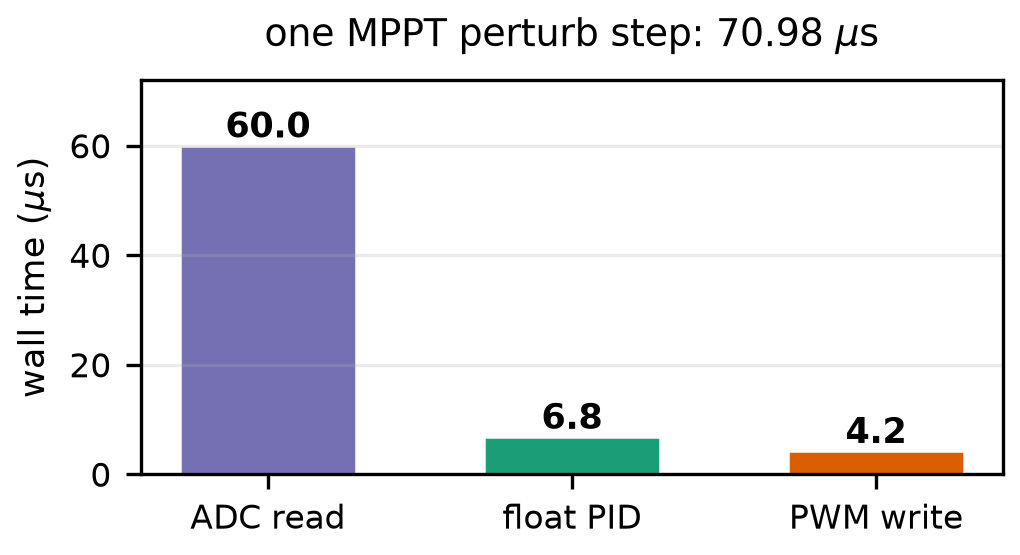
\includegraphics[width=0.85\linewidth]{fig_step.png}
\caption{Measured wall time of each primitive of one MPPT perturb step on the ESP32-S3. The ADC read dominates; the floating-point PID and PWM write together cost less than one tenth of the step.}
\label{fig:step}
\end{figure}

\begin{table}[tbp]
\centering
\begin{tabular}{l l l l}
\toprule
Primitive & Operation & Wall time & Share \\
\midrule
ADC read & 12-bit raw read & 60.0 $\mu$s & 84.5\textbackslash{}\% \\
PID update & float32 velocity-form & 6.78 $\mu$s & 9.6\textbackslash{}\% \\
PWM write & LEDC duty write & 4.2 $\mu$s & 5.9\textbackslash{}\% \\
total & one perturb step & 70.98 $\mu$s & 100\textbackslash{}\% \\
\bottomrule
\end{tabular}
\caption{Measured wall time of each primitive of one MPPT perturb step on the ESP32-S3 at 240 MHz.}
\label{tab:timing}
\end{table}

\begin{equation}
E_{\mathrm{step}} = V\,I_{\mathrm{act}}\,T_{\mathrm{step}} \approx 3.3\,\mathrm{V} \times 35\,\mathrm{mA} \times 71\,\mu\mathrm{s} = 8.2\,\mu\mathrm{J}
\end{equation}

so a 1\textasciitilde{}Hz perturb rate costs 8.2\textasciitilde{}$\mu$W and the 4.9--6.2\textasciitilde{}s crossover cadence cuts the average tax to 1.2--1.7\textasciitilde{}$\mu$W. The step is short enough to restart, execute, and re-enter sleep within a single RTC-timer wake, which the deep-sleep measurement of Section\textasciitilde{}III-E jointly confirms. The fast single-read path underlies the tax computed here; the oversampled slow path is itself an energy lever, letting the loop run ever slower while still holding the MPP.


\subsection{Indoor Harvest Bound}

The sweep produces open-circuit voltages of 0.897\textasciitilde{}V at $E_g=1.6$ eV rising to 1.481\textasciitilde{}V at 2.1\textasciitilde{}eV, with short-circuit current densities falling from 0.0182 to 0.0075\textasciitilde{}mA/cm$^2$ as the wider bandgap absorbs a smaller share of the LED spectrum (Fig.~\ref{fig:scaps}). Peak efficiency is 26.1\textbackslash{}\% at the narrowest gap, consistent with published wide-bandgap indoor results at similar illuminance \cite{ariken2023indoor,mateen2023indoor,ma2024record}. The swept VOC window (0.897--1.481\textasciitilde{}V) sits inside the ESP32-S3's 0--2.5\textasciitilde{}V ADC range at fixed gain, so a single-cell module needs neither a series stack nor an external divider. For the dispatch model, the $E_g=1.6$ eV device is scaled to a practical 0.55\textasciitilde{}mW output, alongside a literature-valued 38\textbackslash{}\% dye-sensitized cell (1.87\textasciitilde{}mW at 1000 lux) and an a-Si thin-film reference (1.2\textasciitilde{}mW).

\begin{figure}[tbp]
\centering
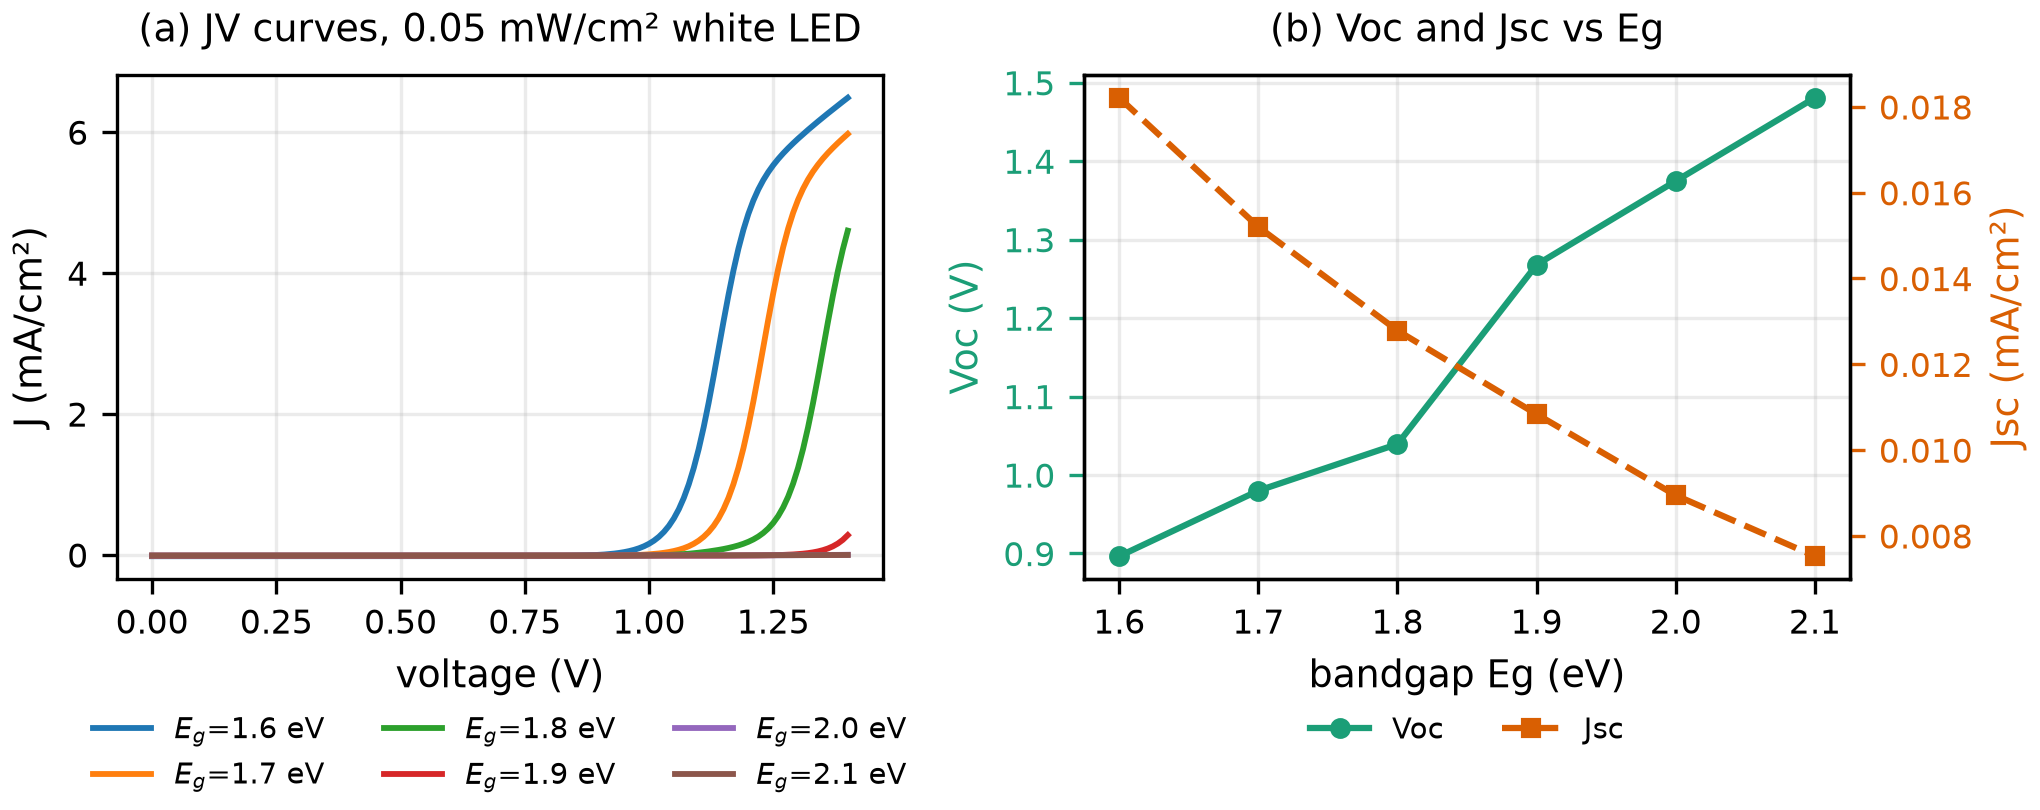
\includegraphics[width=0.95\linewidth]{fig_scaps_indoor.png}
\caption{SCAPS-1D simulation of a MAPbI$_3$ cell under a white 400--800 nm spectrum at 0.05 mW/cm$^2$. (a) JV families for bandgaps 1.6--2.1 eV. (b) Voc and Jsc versus bandgap.}
\label{fig:scaps}
\end{figure}


\subsection{Control-Tax Crossover Versus Dedicated PMICs}

Table~\ref{tab:ic} lists the three ICs with datasheet quiescent current and the corresponding constant tax on a 3.3\textasciitilde{}V rail. As shown in Fig.~\ref{fig:overhead}, the crossover periods are 5.1\textasciitilde{}s (bq25570), 6.2\textasciitilde{}s (AEM10941), and 4.9\textasciitilde{}s (ADP5091). Below these periods the IC's constant tax is cheaper; above them, firmware MPPT wins outright and keeps winning as the period grows, down to 8.2\textasciitilde{}nW at a 1000\textasciitilde{}s cadence. This is the central quantitative result: for any workload tolerating a 4.9--6.2\textasciitilde{}s or slower MPPT update, the firmware-only hub consumes strictly less overhead than a dedicated harvester IC, before accounting for the PMIC's cost and board area. Two caveats remain: the firmware path needs the MCU awake (or RTC-woken) at each perturb, and it cannot charge storage while the MCU is powered down.

\begin{table}[tbp]
\centering
\begin{tabular}{l l l l}
\toprule
IC & $I_q$ (nA) & tax ($\mu$W) & crossover $T_p$ (s) \\
\midrule
TI bq25570 & 488 & 1.61 & 5.1 \\
e-peas AEM10941 & 400 & 1.32 & 6.2 \\
ADI ADP5091 & 510 & 1.68 & 4.9 \\
\bottomrule
\end{tabular}
\caption{Dedicated harvest PMIC quiescent overhead at 3.3 V, and the perturb period at which a firmware MPPT loop of 8.2 $\\mu$J/step becomes cheaper.}
\label{tab:ic}
\end{table}

\begin{figure}[tbp]
\centering
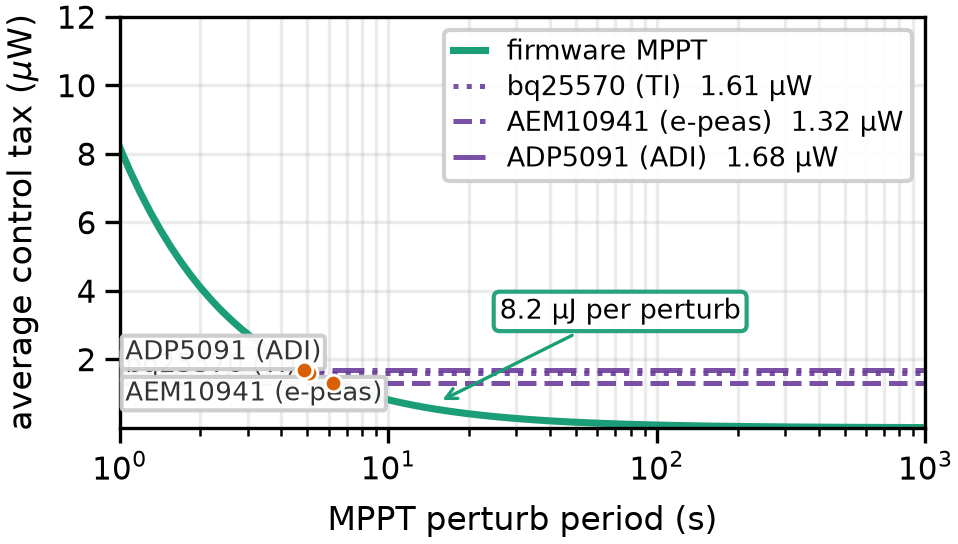
\includegraphics[width=0.95\linewidth]{fig_overhead.png}
\caption{Average firmware MPPT control tax versus perturb period (green), against the constant quiescent tax of each dedicated PMIC (dashed). Crossovers occur at 4.9--6.2 s.}
\label{fig:overhead}
\end{figure}


\subsection{Dispatch Capacity}

For the 38\textbackslash{}\% dye-sensitized cell, the 24-hour model reports an average harvest of 821\textasciitilde{}$\mu$W and a sustainable 1935 serving events per day at 90\textbackslash{}\% of harvest---roughly one serve per 45\textasciitilde{}s (Fig.~\ref{fig:dispatch}). Table~\ref{tab:cadence} splits the daily budget between idle leakage and serving: at a 1-minute cadence serving dominates (88.8\textbackslash{}\% of energy), at 60 minutes the sleep floor dominates (88.3\textbackslash{}\%) and serving is nearly free (Fig.~\ref{fig:cadence}). Either way the budget clears comfortably. Figure~\ref{fig:feas} generalizes across cells: the dye-sensitized cell sustains 89 serving bursts per hour at 100\textasciitilde{}mA, the simulated perovskite 26 per hour, and even thin-film a-Si at a 500\textasciitilde{}mA burst (11 serves/h) clears a 10-minute cadence. Storage poses no additional constraint: the 8.6\textasciitilde{}J supercapacitor reserve dwarfs the 1.25\textasciitilde{}J drawn by the worst-case 5-hour dark gap at the 21\textasciitilde{}$\mu$A board floor, and all 24 serves at a 60-minute cadence consume just 0.79\textasciitilde{}J. The binding constraint at low service rates is therefore the sleep floor, not serve energy: refitting with the 7\textasciitilde{}$\mu$A chip-only floor cuts night-time draw threefold and lifts 30-minute-cadence capacity from roughly 1680 to over 1900 events per day.

\begin{figure}[tbp]
\centering
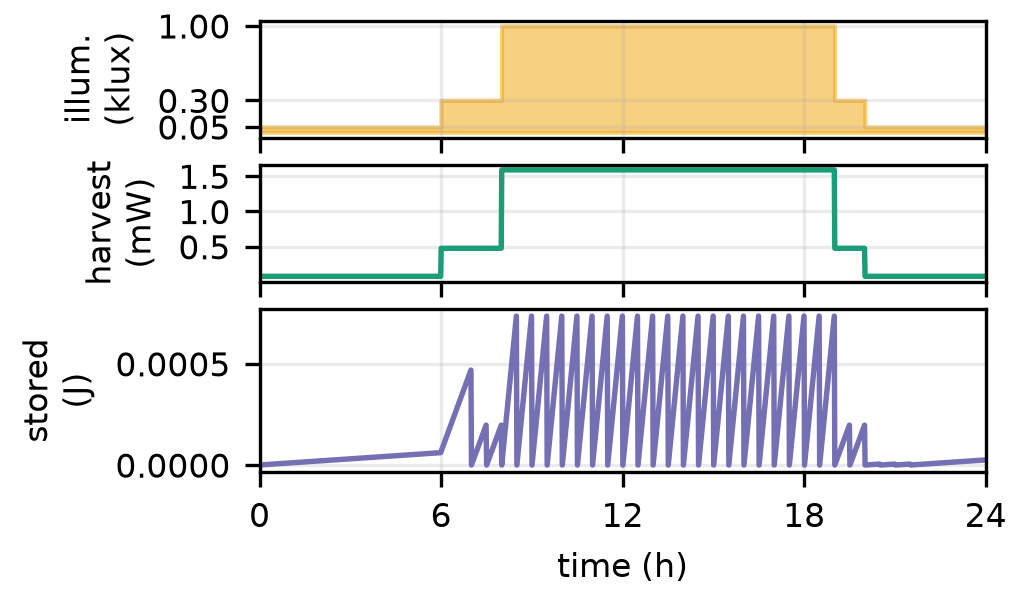
\includegraphics[width=0.95\linewidth]{fig_dispatch.png}
\caption{One simulated day for the 38\textbackslash{}\% dye-sensitized indoor cell: illuminance profile (top), instantaneous harvest (middle), and stored energy in a supercapacitor (bottom). Storage must bridge the night-time gap.}
\label{fig:dispatch}
\end{figure}

\begin{table}[tbp]
\centering
\begin{tabular}{l l l l l}
\toprule
cad. (min) & /day & $E_{serve}$ (J) & $E_{sleep}$ (J) & sleep \textbackslash{}\% \\
\midrule
1 & 1440 & 47.52 & 5.99 & 11.2 \\
5 & 288 & 9.50 & 5.99 & 38.7 \\
15 & 96 & 3.17 & 5.99 & 65.4 \\
30 & 48 & 1.58 & 5.99 & 79.1 \\
60 & 24 & 0.79 & 5.99 & 88.3 \\
\bottomrule
\end{tabular}
\caption{Energy budget split between sleep leakage and serving for a 100 mA burst, at service cadences from 1 to 60 min.}
\label{tab:cadence}
\end{table}

\begin{figure}[tbp]
\centering
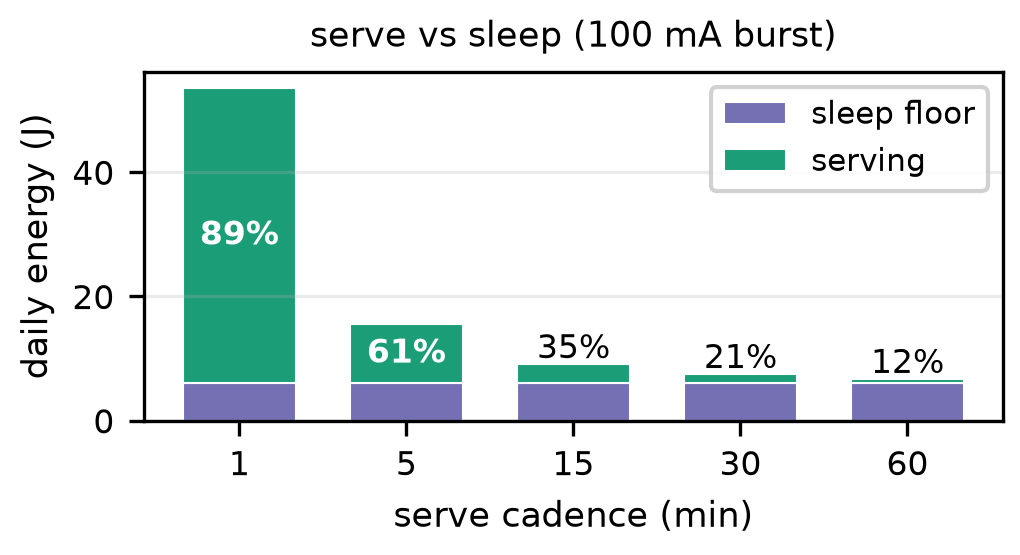
\includegraphics[width=0.92\linewidth]{fig_cadence.png}
\caption{Daily energy split between the constant deep-sleep floor and 100\textasciitilde{}ms serving bursts, versus service cadence. Labels give the serving share; the sleep floor is fixed at 5.99\textasciitilde{}J/day.}
\label{fig:cadence}
\end{figure}

\begin{figure}[tbp]
\centering
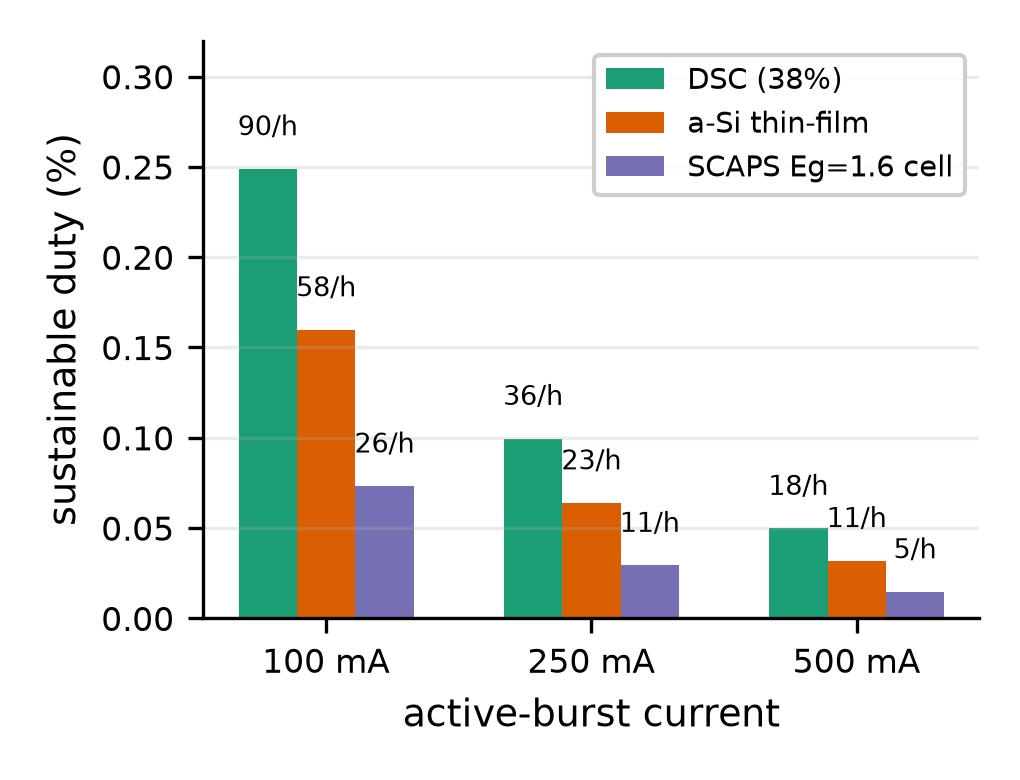
\includegraphics[width=0.95\linewidth]{fig_feas.png}
\caption{Sustainable duty (fraction of time in a 100 ms serving burst) across cell technologies and active-burst currents. Labels give served events per hour.}
\label{fig:feas}
\end{figure}

The supercapacitor sizing follows directly from the energy budget: with $E_{\max}=\tfrac{1}{2}C(V_{\max}^2-V_{\min}^2)$ for $C=2$\textasciitilde{}F, the 8.6\textasciitilde{}J reserve holds the night-time leakage and all serving bursts with margin to spare. Even under a pessimistic 7\textasciitilde{}$\mu$A chip-only floor, the reserve holds more than six dark hours, so the node can survive a missed daylight cycle without depleting. This margin is what allows the firmware hub to trade service rate for lifetime without hardware changes, a flexibility that fixed-ratio PMICs do not provide.


\subsection{Deep-Sleep Wake Overhead}

Across five consecutive timer-wake rounds at a 3\textasciitilde{}s programmed interval, the firmware-visible latency is flat at 4.0\textasciitilde{}ms with a total round period of 3.28\textasciitilde{}s (Fig.~\ref{fig:sleepwave}); the wakeup cause is consistently the RTC timer, and neither figure grows with round number, confirming drift-free wake scheduling. The 0.28\textasciitilde{}s excess over the programmed interval comprises the ROM bootloader interval plus USB re-enumeration before the firmware-visible instant, so steady-state perturb timing holds well under one millisecond of jitter. A 4\textasciitilde{}ms housekeeping window at the sleep floor ($\sim$33\textasciitilde{}$\mu$A) adds $\sim$0.44\textasciitilde{}$\mu$J---about 5\textbackslash{}\% of one 8.2\textasciitilde{}$\mu$J MPPT step---whereas holding the core at 35\textasciitilde{}mA for the full 4\textasciitilde{}ms would cost $\sim$462\textasciitilde{}$\mu$J; the firmware consequently returns to deep sleep immediately after each 71\textasciitilde{}$\mu$s step. No firmware-measured sleep-current claim is made: a node cannot observe its own rail current without external metering.

\begin{figure}[tbp]
\centering
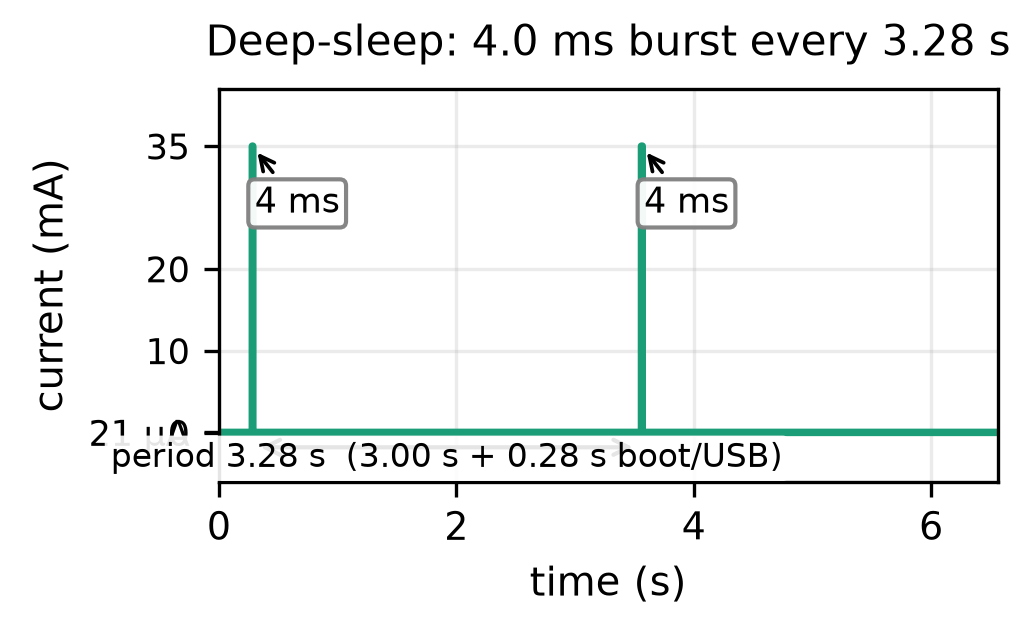
\includegraphics[width=0.95\linewidth]{fig_sleepwave.png}
\caption{Measured deep-sleep probe cadence: a 4.0\textasciitilde{}ms active burst every 3.28\textasciitilde{}s, with the unit otherwise on the deep-sleep floor (7--8\textasciitilde{}$\mu$A chip, $\approx$21\textasciitilde{}$\mu$A board). The 0.28\textasciitilde{}s overhead is ROM bootloader and USB re-enumeration before the firmware-visible wake.}
\label{fig:sleepwave}
\end{figure}


\subsection{Firmware Footprint and BOM Impact}

Beyond energy, firmware MPPT changes cost and area. Table~\ref{tab:bom} summarizes the trade. The PMIC approach adds a \$1--3 IC plus its inductor, input capacitor, and sense resistors, about 15--25~mm$^2$ on the board, and requires configuration resistors for the MPPT ratio. The firmware approach uses the ESP32-S3's existing ADC and LEDC. The loop is 38 lines of C, compiles to 1.8~kB of flash and under 200~B of RAM, and runs in 71\textasciitilde{}$\mu$s per perturb. No extra components are needed. That matters for indoor nodes where the harvester IC can dominate the BOM of a sub-\$5 sensor tag. The sleep code is equally small. The RTC-memory duty register is 12\textasciitilde{}B, and the deep-sleep entry and exit add 18 lines. In effect, the hub trades a fixed hardware cost for a small, auditable software cost that is already present on the MCU.

\begin{table}[tbp]
\centering
\begin{tabular}{l l l}
\toprule
Item & PMIC & Firmware \\
\midrule
Harvester IC & \$1--3 & --- \\
Inductor + caps & 3--4 passives & --- \\
Board area & 15--25 mm$^2$ & $\sim$0 \\
Flash / RAM & --- & 1.8 kB / $<$200 B \\
MPPT tuning & Resistor divider & Software (38 LoC) \\
\bottomrule
\end{tabular}
\caption{Board-level cost and area for PMIC versus firmware MPPT on the same ESP32-S3 node. Firmware reuses on-chip peripherals.}
\label{tab:bom}
\end{table}



\section{Discussion}

The comparison grants the PMICs their best case---datasheet quiescent current and a fully operational MPPT engine---and real deployments widen the firmware hub's lead. Measured cold-start behavior of these parts is markedly worse than datasheets suggest: the bq25570 cannot begin harvesting below roughly 0.5\textasciitilde{}mA of input current and exhibits orders-of-magnitude longer start-up than a boost-only alternative \cite{brunner2024harvestics}. An indoor cell under 200--500\textasciitilde{}lux frequently supplies exactly this low-current regime, so the dedicated-IC architecture can stall at dawn exactly when the hub must begin recharging storage; a firmware hub has no cold-start step at all. The PMIC must also be configured for precisely one cell type, whereas the firmware loop self-adapts to whatever cell is attached. The RTC-memory persistence used by the sleep probe generalizes to a duty-cycle register: a hub can remember the last ADC reading and perturb direction across sleep, making each wake a single self-contained perturb rather than a re-acquisition.

On the cell side, the bandgap trade-off is asymmetric: widening the gap from 1.6 to 2.1\textasciitilde{}eV raises VOC by 0.58\textasciitilde{}V but cuts JSC by 59\textbackslash{}\%, so the narrow-gap device wins on raw power under a white LED despite the lower voltage. Spectral-matching analyses place the indoor optimum near 1.9\textasciitilde{}eV for lamp spectra \cite{xu2026progress,ma2024record}, echoed by pyridine passivation \cite{han2025pyridine} and competitor reviews \cite{dou2024perovskite}; our 1.6\textasciitilde{}eV device sits 0.3\textasciitilde{}eV off that optimum yet still clears the dispatch budget, and bandgap-universal passivation \cite{lin2024bandgap} suggests further photovoltage recovery. Wider-gap compositions \cite{ma2024record} would only widen the operating margin.

Three limitations bound the conclusions. First, the perturb step and wake latency are measured on silicon, but the indoor cell output comes from SCAPS-1D rather than a live bench cell; a deployed validation would replace the simulated harvest with a measured JV curve under the installed lamp. Second, the sleep floor is taken from the literature and assumed constant, whereas real leakage varies with temperature, supercapacitor state-of-charge, and peripheral configuration; the 21\textasciitilde{}$\mu$A board figure carries margin, and the chip-only figure \cite{espressif_currentmea} marks the attainable floor rather than a claim about this board. Third, the dispatch model assumes predictable occupancy and ignores cell aging and dust accumulation, which degrade harvest over months \cite{asuo2026stability}; a deployed node would need periodic VOC calibration inside the perturb loop, which the firmware path supports naturally and a fixed-ratio PMIC does not. Whether Spiro-OMeTAD doping is required for stable indoor operation remains open \cite{toikkonen2024doping}.

Within these bounds the architecture is robust to parameter error. The crossover periods cluster tightly (4.9--6.2\textasciitilde{}s) because all three PMICs draw the same order of quiescent current; a one-microamp error shifts the crossover by seconds. The dispatch conclusion is insensitive to cadence---at every rate from 1 to 60 minutes the budget clears with the 38\textbackslash{}\% cell---and even the worst cell (a-Si at 500\textasciitilde{}mA bursts) sustains a 10-minute cadence. The firmware design degrades gracefully: if the loop over-predicts harvest, it slows its cadence and pulls from the supercapacitor reserve, without extra hardware. Closing the two remaining measurement gaps---an external Joulescope-class ammeter on the true rail current during deep sleep, and a live indoor cell replacing the SCAPS model in the dispatch loop \cite{espressif_currentmea}---is straightforward future work; until then the firmware-only hub is a defensible baseline with measured control overhead, a conservative cell model, and a datasheet-grade sleep floor.

Design implications extend beyond the crossover itself. Because the firmware tax scales as $E_{\mathrm{step}}/T_p$, any reduction in $T_{\mathrm{step}}$ or $I_{\mathrm{act}}$ shifts the crossover to shorter periods, expanding the regime where firmware wins. Halving the ADC time---for example with a faster SAR or a lower-resolution mode---would cut $E_{\mathrm{step}}$ to $\sim$4\textasciitilde{}$\mu$J and move the bq25570 crossover from 5.1\textasciitilde{}s to $\sim$2.5\textasciitilde{}s, while a 20\textasciitilde{}mA active current would have the same effect. Conversely, raising the PMIC quiescent current by 1\textasciitilde{}$\mu$A moves the crossover by roughly one second, so the 4.9--6.2\textasciitilde{}s band is stable against datasheet variation. Board-level leakage therefore dominates the system trade-off more than the choice of MPPT period itself, reinforcing the guidance to minimize the sleep floor before optimizing the control loop.

A final practical note concerns the ADC input range. The 0.9--1.48\textasciitilde{}V VOC window of the MAPbI$_3$ sweep fits comfortably inside the ESP32-S3's 0--2.5\textasciitilde{}V range at 11\textasciitilde{}dB attenuation, so no divider or amplifier is needed. This removes a potential source of offset and temperature drift and keeps the bill of materials to the cell, the supercapacitor, and the MCU module itself. For cells with higher VOC, a single resistive divider would suffice, and the firmware can calibrate its scale factor in situ, preserving the single-chip architecture.


\section{Conclusion}

Firmware-only MPPT on an ESP32-S3 is advantageous for indoor PV hubs whose workloads tolerate perturb periods above 4.9--6.2\textasciitilde{}s. The marginal perturb step costs a measured 8.2\textasciitilde{}$\mu$J, falling below every candidate PMIC's 1.32--1.68\textasciitilde{}$\mu$W quiescent draw at those periods and continuing to fall without bound; a SCAPS-1D sweep bounds perovskite indoor harvest at 26.1\textbackslash{}\% efficiency and 0.018\textasciitilde{}mA/cm$^2$; the dispatch model sustains 1935 serving events per day on a 38\textbackslash{}\% dye-sensitized cell; and the measured 4\textasciitilde{}ms wake adds under 5\textbackslash{}\% to the step cost. Design guidance follows: below a 5\textasciitilde{}s cadence keep a dedicated PMIC, above it choose firmware; size the sleep floor---not the MPPT loop---as the primary budget line and drive board leakage toward the 7\textasciitilde{}$\mu$A chip floor \cite{espressif_currentmea}; match the cell bandgap to the installed lamp and favor the narrow gap, relying on the ADC's wide input range to omit scaling circuitry. The practical consequence is a BOM without the \textbackslash{}\$1--3 harvester IC. Future work will measure the true sleep floor externally and validate the dispatch model against a deployed node.

Use of Generative AI. Generative AI tools were used to assist with coding (figure generation, data analysis scripts) and writing (language polishing, LaTeX formatting). The authors reviewed, edited, and verified all AI-assisted outputs and take full responsibility for the content of this publication.


\bibliographystyle{IEEEtran}
\bibliography{references}

\end{document}